\section{Definição do problema}

A Lei n.º 13.589/2018 obriga edifícios de uso público a manter um Plano de Manutenção, Operação e Controle (PMOC) dos sistemas de climatização \cite{brasil2018lei}. Na Assembleia Legislativa do Ceará (ALECE), a manutenção preventiva cobre mais de mil aparelhos (\textit{split hi-wall}, piso-teto e cassete) em quatro prédios (SEDE e Anexos I, II e III), executada por 7 equipes de 2 técnicos, das 9h às 17h. O sistema de gestão do PMOC agenda cada ciclo com uma regra simples: cada prédio tem um número fixo de \textit{vagas por dia}, preenchidas em ordem de cadastro. A regra trata todos os aparelhos como iguais e ignora o deslocamento entre prédios, de modo que o plano promete menos dias do que o ciclo realmente leva.

\textbf{Modelo.} Sejam $J$ os aparelhos, $K$ as equipes (idênticas), $D$ os dias e $b_j$ o prédio do aparelho $j$, com tempo de manutenção $p_j$. A jornada útil é $H=420$ min. O deslocamento de $b$ para $b'$ é $s_{bb'}$, com $s_{bb}=5$ min para troca de sala, e cada dia começa na SEDE ($b=0$). O prédio $b$ aceita até $c_b$ aparelhos por dia. As variáveis são: $x_{jkd}=1$ se $j$ é atendido pela equipe $k$ no dia $d$; $z_{jkd}=1$ se $j$ é o primeiro da equipe $k$ no dia $d$; $y_{ijkd}=1$ se $j$ sucede $i$; $S_j$ é o início do atendimento de $j$ no dia; e $C_{\max}$ é o \textit{makespan} em minutos úteis acumulados.
\begin{align}
\min\; & C_{\max} \nonumber\\
\text{s.a.}\; & \textstyle\sum_{k,d} x_{jkd} = 1, \qquad z_{jkd} + \sum_{i\neq j} y_{ijkd} = x_{jkd}, \qquad \sum_{l\neq j} y_{jlkd} \le x_{jkd} && \forall j,k,d \label{eq:atrib}\\
& \textstyle\sum_{j} z_{jkd} \le 1 && \forall k,d \label{eq:inicio}\\
& S_j \ge s_{0b_j}, \qquad S_j + p_j \le H && \forall j \label{eq:janela}\\
& \textstyle S_j \ge S_i + p_i + s_{b_ib_j} - M_{ij}\bigl(1-\sum_{k,d} y_{ijkd}\bigr) && \forall i\neq j \label{eq:seq}\\
& \textstyle\sum_{j:\,b_j=b}\sum_k x_{jkd} \le c_b && \forall b,d \label{eq:vagas}\\
& \textstyle C_{\max} \ge \sum_{k,d} dH\,x_{jkd} + S_j + p_j && \forall j \label{eq:cmax}
\end{align}
As restrições \eqref{eq:atrib}--\eqref{eq:inicio} formam uma sequência por equipe e dia, \eqref{eq:janela} impõe a saída da SEDE e a jornada, \eqref{eq:seq} encadeia os tempos e elimina subciclos (com $M_{ij}=H+s_{b_ib_j}-s_{0b_j}$), \eqref{eq:vagas} limita as vagas por prédio e \eqref{eq:cmax} define o \textit{makespan}. Acrescentam-se a quebra de simetria $\sum_j x_{jkd}\ge\sum_j x_{j,k+1,d}$ e duas desigualdades válidas, com $\bar s_j$ o menor deslocamento até $j$: $\sum_j (p_j+\bar s_j)x_{jkd}\le H$ e $C_{\max}\ge dH\sum_j z_{jkd}+\sum_j(p_j+\bar s_j)x_{jkd}$. As equipes são máquinas paralelas, os aparelhos são tarefas e o deslocamento é um tempo de preparação dependente da sequência. O problema generaliza o $P_m|s_{ij}|C_{\max}$, que é NP-difícil \cite{allahverdi2015third,vallada2011genetic}.

\section{Método proposto}

\textbf{Representação e decodificação.} Uma solução é uma permutação $\pi$ dos aparelhos. O decodificador percorre $\pi$ e atribui cada aparelho à equipe que o conclui mais cedo. Se não houver tempo no dia ou vaga no prédio, o aparelho passa ao primeiro dia seguinte com vaga, partindo da SEDE. Assim, toda permutação gera uma programação viável. A avaliação é $f(\pi)=C_{\max}+10^{-7}\sum_k(d_kH+t_k)$, em que o segundo termo só desempata. Para acelerar a busca, a avaliação de inserções reaproveita o estado do prefixo comum e interrompe uma avaliação assim que o $C_{\max}$ parcial supera o melhor valor conhecido, sem alterar o resultado.

\textbf{Heurísticas de referência.} (i) \textit{Regra atual}: reproduz o sistema da ALECE e é executada com os tempos reais e os deslocamentos. (ii) \textit{LPT+NEH}: ordena os aparelhos pelo maior $p_j$ e insere cada um na melhor posição \cite{nawaz1983heuristic}. A LPT+NEH também é a solução inicial das quatro meta-heurísticas.

\textbf{Meta-heurísticas.} \textit{IG} \cite{ruiz2007simple}: remove $d$ aparelhos, reinsere cada um na melhor posição e aceita pioras com probabilidade $e^{-\Delta/T}$, com $T=\tau\sum_jp_j/(10n)$. \textit{VNS} \cite{mladenovic1997variable}: \textit{shaking} com as cinco vizinhanças da aula (troca; inserção no início; bloco de 4 para o início; bloco de 4 para o fim; troca de dois blocos) até $k_{\max}$, e busca local VND amostrada (troca e inserção, \textit{first improvement}) até $L$ tentativas sem melhoria. \textit{ILS} \cite{lourenco2003iterated}: embaralha um trecho de $\lceil \text{int}\cdot n\rceil$ posições, aplica a mesma busca local e aceita soluções melhores ou iguais. \textit{AG} \cite{goldberg1989genetic}: população de tamanho $P$ (a LPT+NEH e cópias perturbadas dela), torneio binário, cruzamento OX \cite{davis1985applying}, mutação por inserção com probabilidade $p_m$ e substituição estacionária do pior indivíduo.

\textbf{Calibração.} Seguiu-se a metodologia da disciplina: 30\% das instâncias (7 de 24), todas as combinações de uma grade por algoritmo, 5 execuções cada e escolha pelo menor desvio médio em relação à melhor solução da instância. As grades foram: IG $d\in\{2,4,6\}\times\tau\in\{0{,}1;0{,}4;0{,}8\}$; VNS $k_{\max}\in\{3,5\}\times L\in\{0{,}5n;n;2n\}$; ILS int $\in\{1;2{,}5;5\}\%\times L\in\{0{,}5n;n;2n\}$; AG $P\in\{20,50,100\}\times p_m\in\{0{,}05;0{,}2\}$. Em seguida, o Optuna \cite{akiba2019optuna} (TPE, 12 tentativas, 2 execuções por instância) explorou intervalos mais amplos, e ficou a melhor configuração entre as duas etapas.

\textbf{Configuração experimental.} Como os dados do sistema são internos, foram geradas 25 instâncias sintéticas com a estrutura real: prédios com 40/25/20/15\% dos aparelhos; tipos \textit{hi-wall} (60\%), piso-teto (25\%) e cassete (15\%), com tempos de 40--65, 60--85 e 75--100 min conforme o porte (BTU) e o acesso; deslocamentos de 8 a 20 min; e vagas diárias 30\% acima da distribuição uniforme. A ALECE-base ($n=1050$, $m=7$) representa o caso real. As demais combinam $n\in\{1000,1250,1500,2000\}$ e $m\in\{5,7\}$, com 3 réplicas. Nas 18 instâncias de teste, cada meta-heurística foi executada 30 vezes, com $0{,}006n$ s de CPU (6 a 12 s); a busca local inicial do VNS e do ILS (até 4\% desse tempo) não é contada. Para validar o método, o modelo (1)--(6) foi resolvido com o CBC (Python-MIP) em 16 instâncias pequenas ($n=5$ a $8$, $m\in\{1,2\}$), e cada meta-heurística foi executada 10 vezes por 1 s em cada uma. A implementação foi feita em Python 3.12 com Numba, em um notebook de 4 núcleos lógicos. Código, instâncias e resultados estão em \url{https://github.com/JovannaPi/pmoc-po2}.

\section{Análise e discussão dos resultados}

\textbf{Validação exata.} O CBC provou a otimalidade nas 16 instâncias pequenas. O tempo médio passou de 0,15 s com $n=5$ para 52,6 s com $n=8$, o que mostra o crescimento explosivo que inviabiliza o modelo exato na escala real. Com os parâmetros calibrados, as meta-heurísticas atingiram o ótimo em todas as instâncias, em 639 das 640 execuções (só uma execução do ILS não o encontrou). Isso mostra que o decodificador não exclui as soluções ótimas nessas instâncias e que os métodos as encontram.

\textbf{Calibração.} A \autoref{fig:calib} mostra a grade. O Optuna melhorou o IG ($d=2$, $\tau=1{,}08$; desvio de 0,61\% para 0,49\%) e o VNS ($k_{\max}=2$, $L=2{,}4n$; de 0,51\% para 0,49\%). Para o ILS (int $=1\%$, $L=0{,}5n$) e o AG ($P=100$, $p_m=0{,}05$), a grade foi melhor. Destruições e perturbações pequenas funcionaram melhor, o que é coerente com a escala: com mais de mil aparelhos, mexer em poucos de cada vez preserva a estrutura da solução.

\begin{figure}[!htbp]
    \centering
    \caption{\label{fig:calib} Calibração por grade: desvio percentual relativo por combinação (7 instâncias, 5 execuções). Em vermelho, a melhor combinação.}
    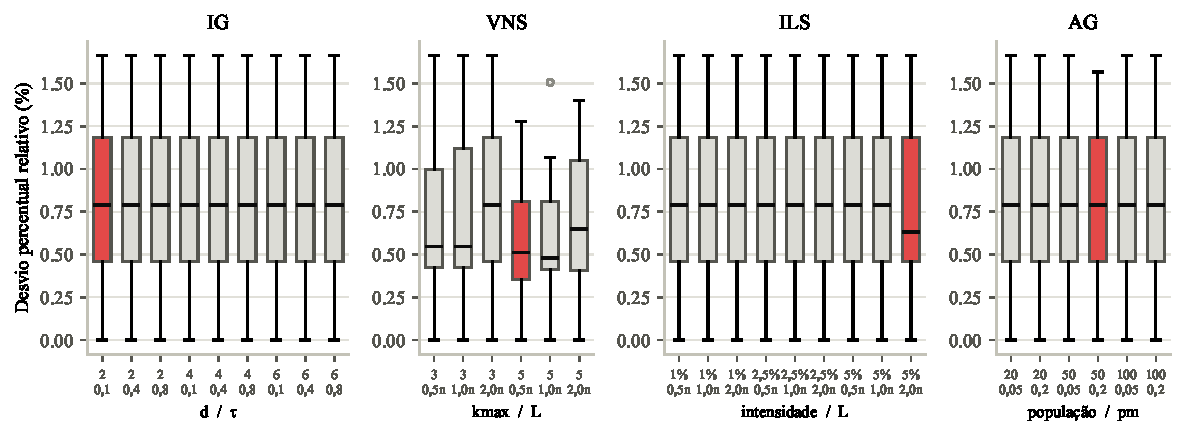
\includegraphics[width=\textwidth]{figuras/calibracao_boxplot.pdf}
\end{figure}

\textbf{Comparação.} A \autoref{tab:rpd} mostra o RPD em relação à melhor solução conhecida. As meta-heurísticas ficam, em média, a 0,2--0,35\% dela, contra 6,1\% da regra atual e 0,66\% da LPT+NEH. Os RPDs não são normais (Shapiro-Wilk, $p<10^{-23}$), então seguiu-se o caminho não paramétrico \cite{derrac2011practical}. O teste de Kruskal-Wallis aponta diferença ($H=41{,}2$; $p=5{,}9\times10^{-9}$), e o pós-teste de Dunn (Bonferroni) separa dois grupos: ILS e VNS são melhores que IG e AG ($p<0{,}001$), sem diferença dentro de cada grupo. Como as 30 execuções de uma instância não são independentes, aplicou-se também o teste de Friedman, com as instâncias como blocos \cite{demsar2006statistical}: $Q=17{,}5$, $p=5{,}5\times10^{-4}$, com postos médios ILS 1,92, VNS 2,14, IG 2,42 e AG 3,53. Pelo pós-teste de Nemenyi, apenas o AG difere dos demais ($p<0{,}05$). O ILS é, portanto, o mais consistente, e as diferenças diminuem com o tamanho: com $n=2000$, os quatro métodos ficam abaixo de 0,13\%.

\begin{table}[htb]
    \centering
    \caption{\label{tab:rpd} RPD médio (\%) e taxa de sucesso (TS, \% das execuções com RPD $\le 1\%$) por número de aparelhos (30 execuções por instância). $^*$ALECE-base.}
    \small
    \begin{tabular}{lrrrrrrrrrr}
        \toprule
        & \multicolumn{6}{c}{RPD médio (\%)} & \multicolumn{4}{c}{TS (\%)} \\
        \cmidrule(lr){2-7}\cmidrule(lr){8-11}
        $n$ & Regra atual & LPT+NEH & IG & VNS & ILS & AG & IG & VNS & ILS & AG \\
        \midrule
        1000 & 6,20 & 1,99 & 0,90 & 0,68 & 0,59 & 0,81 & 61 & 81 & 92 & 60 \\
        1050$^*$ & 6,22 & 1,56 & 0,86 & 0,35 & 0,36 & 0,39 & 70 & 100 & 100 & 100 \\
        1250 & 6,08 & 0,36 & 0,21 & 0,21 & 0,16 & 0,29 & 100 & 100 & 100 & 100 \\
        1500 & 5,95 & 0,40 & 0,26 & 0,11 & 0,13 & 0,14 & 100 & 100 & 100 & 100 \\
        2000 & 6,25 & 0,13 & 0,10 & 0,10 & 0,09 & 0,12 & 100 & 100 & 100 & 100 \\
        \midrule
        Média & 6,10 & 0,66 & 0,35 & 0,24 & 0,22 & 0,30 & 92 & 97 & 99 & 93 \\
        \bottomrule
    \end{tabular}
\end{table}

\textbf{Iterações.} A \autoref{fig:conv} mostra a convergência na ALECE-base. O VNS faz poucas iterações, pois cada busca local é cara, mas já parte de uma solução muito boa. O ILS faz cerca de 100 iterações, com ganhos pequenos e contínuos. O AG evolui por mais de 1500 gerações e se aproxima dos dois. O IG melhora mais devagar e varia mais entre execuções, o que explica a sua maior dispersão.

\begin{figure}[!htbp]
    \centering
    \caption{\label{fig:conv} Convergência na ALECE-base: mediana (linha) e intervalo interquartil (faixa) do melhor $C_{\max}$ das 30 execuções, por iteração.}
    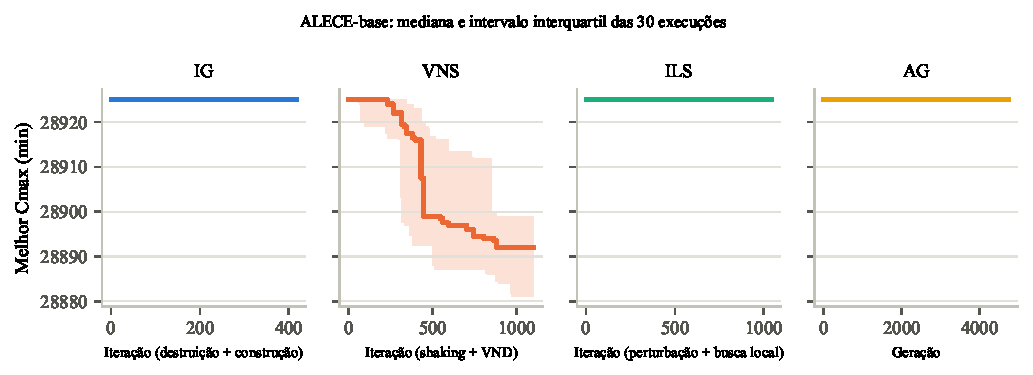
\includegraphics[width=0.95\textwidth]{figuras/convergencia_iteracoes.pdf}
\end{figure}

\textbf{Impacto prático.} Na ALECE-base, o sistema promete 19 dias, mas a regra atual leva 28 quando se consideram os tempos reais e os deslocamentos. As meta-heurísticas fecham o ciclo em 26 dias (todas as execuções de VNS, ILS e AG) e reduzem o deslocamento em cerca de 7\%. O limite inferior é de 24 dias (carga total dividida pelas equipes). Em todas as instâncias, os métodos reduzem o $C_{\max}$ da regra atual em 5,5\%, cerca de 2,5 dias por ciclo. A \autoref{fig:impacto}b mostra ainda que nem com 9 equipes o ciclo cabe nos 19 dias do plano: o número de dias do sistema é otimista por construção, e um planejamento confiável precisa do tempo de cada aparelho.

\begin{figure}[!htbp]
    \centering
    \caption{\label{fig:impacto} ALECE-base: (a) aparelhos concluídos por dia; (b) dias do ciclo conforme o número de equipes.}
    \begin{subfigure}[b]{0.52\textwidth}
        \centering
        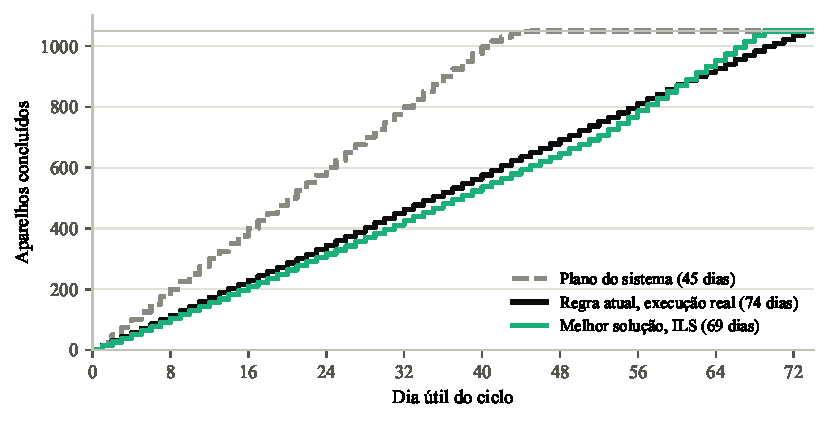
\includegraphics[width=\textwidth]{figuras/curva_conclusao_alece.pdf}
        \caption{Plano, regra atual e melhor solução}
    \end{subfigure}
    \hfill
    \begin{subfigure}[b]{0.46\textwidth}
        \centering
        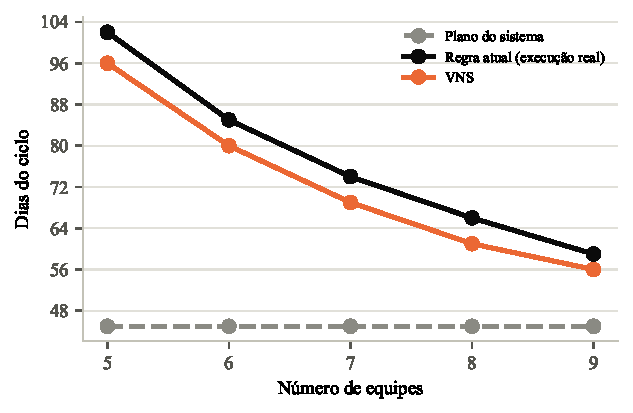
\includegraphics[width=\textwidth]{figuras/sensibilidade_equipes.pdf}
        \caption{Sensibilidade (ILS)}
    \end{subfigure}
\end{figure}

\section{Conclusões}

Este trabalho modelou a programação da manutenção preventiva (PMOC) dos aparelhos de ar-condicionado da ALECE como um problema de máquinas paralelas com tempos de preparação dependentes da sequência, jornada diária e limite de vagas por prédio. Foram propostos um modelo de programação inteira mista e quatro meta-heurísticas (IG, VNS, ILS e AG), calibradas pela metodologia da disciplina com refinamento pelo Optuna.

O modelo exato confirmou que as meta-heurísticas encontram o ótimo nas instâncias pequenas, mas o seu tempo cresce rápido demais para a escala real. Com mais de mil aparelhos, ILS e VNS foram os métodos mais eficazes, com diferença estatisticamente significativa em relação ao IG e ao AG. Na prática, o plano atual subestima o ciclo em 9 dias no caso de referência. As meta-heurísticas encurtam o ciclo em 2 dias em relação à execução real da regra atual e permitem dimensionar quantas equipes são necessárias para um prazo desejado.

Como limitação, as instâncias são sintéticas, porque os dados do sistema são internos. Como trabalhos futuros, sugerem-se: (i) estimar os tempos com um estudo de tempos em campo; (ii) incluir a periodicidade das tarefas do PMOC e as restrições de dia por setor; (iii) desenvolver uma matheurística que use o modelo exato para reotimizar dias; e (iv) integrar o método ao módulo de cronograma do sistema.
